\documentclass[12pt,a4paper]{article}

\usepackage[utf8]{inputenc}
\usepackage[spanish,activeacute]{babel}
\selectlanguage{spanish}
\usepackage{amsmath}
\usepackage{amsfonts}
\usepackage{amssymb}
\usepackage[font=scriptsize,labelfont=bf]{caption}

\usepackage{multirow}
\usepackage{graphicx}

\usepackage[left=4cm,right=4cm,top=4cm,bottom=4cm]{geometry}
\usepackage{listings} 
\usepackage{tikz}
\usepackage{enumerate}

\usetikzlibrary{arrows}


\newlength{\margen}
\setlength{\margen}{\paperwidth}
\addtolength{\margen}{-\textwidth}
\setlength{\margen}{0.5\margen}
\addtolength{\margen}{-1in}
\setlength{\oddsidemargin}{\margen}
\setlength{\evensidemargin}{\margen}


\title{Sistemas Distribuidos de Procesamiento de Datos\\Práctica Hadoop}
\author{José Vicente Mellado \\ Jon Kobeaga Urriolabeitia\\Universidad Rey Juan Carlos}

\begin{document}

\maketitle
\hrule
\tableofcontents
\newpage
\section{Introducción}
En este documento se explicarán los pasos, el código, las conclusiones y los problemas tenidos a la hora de hacer el análisis de sentimientos de los estados de Estados Unidos. Para llevar acabo dicho análisis se ha utilizado un fichero, llamado \textit{AFIN-en-165}, creado por Finn Årup Nielsen entre los años 2009 y 2015, que nos indica la felicidad que nos aporta cada palabra. La lista fue creada a mano y a cada palabra le corresponde un número entero entre [-5,5].


\section{Descripción del código}

En este apartado explicaremos el código utilizado para hacer el análisis de sentimientos. Se ha dividido en tres fases principales:

\begin{enumerate}
\item Obtención de los datos.
\item Análisis de los datos.
\item Representación de los resultados.
\end{enumerate}

\subsection{Obtención de los datos}
Se ha levantado una insatncia de EC2 para obtener los datos. Los datos obtenidos se han guardado en formato JSON y para su obtención se han utilizado dos criterios diferentes. Por una parte, se ha descargado el 1\% de todos los tweets que se generan en el momento, sin tener en cuenta la localización ni el idioma. De esta forma se han descargado 1,7GB.\\
Por otra parte, se ha hecho un filtrado para descargar los tweets, obteniendo sólo los tweets en inglés y de Estados Unidos. Para ello, al API de Twitter le hemos indicado el área que nos interesa, es decir, le hemos indicado que nos descargue únicamente los tweets generados entre Canadá y México. Quedan excluidos Alaska, las colonias y otras islas. EL estado se guarda en el campo ``usa\_state''. Además, como cada tweet tiene mucha información, sólo hemos guardado los campos que nos interesan, con el objetivo de que se ocupe el menor espacio posible. De esta forma se han descargado 300MB y 500.000 tweets.\\
En total, se ha trabajado con un fichero de 2GB y 829.576 tweets.

\subsection{Análisis de Resultados}

El análisis de resultados consiste en dos scripts, uno con las funciones principales y MapReduceJob y el otro con los métodos que serven para facilitar el trabajo de las funciones principales. El MRJob  consiste en dos pasos que explicaremos a continuación.

\subsubsection{Primer paso}
En este primer paso se ejecutan el mapper, combiner y reducer. Para que se pueda ejecutar el mapper, se necesita tener un diccionario de las palabras y su correspondiente nivel de felicidad. Este diccionario se crea a través del archivo \texttt{AFINN-en-165.txt}. Además, si alguna palabra no está en el diccionario se ha considerado que la felicidad que aporta es nula. Ahora, explicaremos en qué consiste cada función:

\begin{itemize}
\item \textbf{Mapper:} Se lee cada tweet y lo primero que se filtra es el idioma, nos quedamos con los tweets en inglés. Después dependiendo del criterio utilizado para descargar el tweet, hay diferentes campos que nos indican la localización. Si el tweet descargado ya ha sido filtrado, el campo que nos indica el estado es ``usa\_state''. Si el tweet no ha sido filtrado, hay dos campos que nos indican su localización: ``user''$\rightarrow$``location'' y ``place''$\rightarrow$ ``country''. Se ha utilizado la libreria \texttt{us} para obtener el estado partiendo de la información de los campos.\\

Después se ha obtenido el texto del tweet, que nos indica el campo ``text''. Debido a que cada palabra del fichero \textit{AFIN-en-165} está en minúscula, hemos pasado cada palabra a minúscula y solamente hemos cogido los caracteres del alfabeto inglés y ``\#'' que hace referencia a los hashtags.\\

Una vez que se tienen las palabras del tweet, si es un hashtag la pareja \textit{(clave,valor)} que se envía es \textit{(hashtag,1)}. En caso de que no lo sea, se envía \textit{(clave,valor)=(estado,felicidad\_palabra)} 

\item \textbf{Combiner:} Este paso se utiliza para simplificar el trabajo en el reducer. Suma el valor de los hashtags y los estados y los envía como \textit{(hashtag o estado, valor)}.

\item \textbf{Reducer:} Suma el valor de los hashtags y de los estados, pero en este caso, el valor que se envía es una tupla formada por \textit{(valor,hashtag)} o \textit{(valor,estado)}. Esta técnica se utiliza para poder paralelizar el segundo paso del MRJob.

\subsubsection{Segundo paso}

En este segundo paso, se obtienen  la felicidad de cada estado, el estado más feliz y los diez hashtags más utilizados. Para ello, solamente se utiliza el reducer.\\

Se crean dos diccionarios por separado, uno con todos los estados y su respectiva felicidad y otro con todos los hashtags y el número de veces que se han utilizado. Después se ordenan los diccionarios y se coge el estado más feliz y los diez hashtags más comunes.
\end{itemize}

\subsection{Representación de los Datos}
Los resultados obtenidos se han representado en un mapa de colores. Cada estado se ha pintado de un color dependiendo de su nivel de felicidad. Se han utilizado \texttt{ShapeFiles}, para dibujar los estados con sus respectivas fronteras. Para representar los resultados, se ha utilizado la librería \texttt{Basemap}.\\

Se ha escalado la felicidad de cada estado para que a la hora de pintar no haya diferencias grandes. se han escalado de la siguiente forma:
$$hap_{estado}=1-\displaystyle \sqrt{\dfrac{hap-hap_{min}}{hap_{max}-hap_{min}}}$$

donde \textit{hap} indica la felicidad del estado y $hap_{max}\ \text{,}\ hap_{min}$ son el valor máximo y mínimo de felicidad.
El estado más feliz se pinta de azul y el menos feliz de un color amarillo-verdoso.

%\begin{figure}[h]
%\centering
%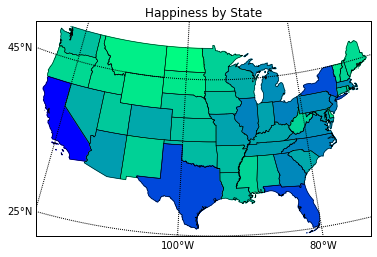
\includegraphics[scale=1]{happiness.png}
%\caption{Gráfico que representa la felicidad de cada estado.}
%\end{figure}

\section{Diferentes Formas de Ejecución}

Se ha ejecutado de cinco formas diferentes:
\begin{enumerate}
\item Local: \texttt{python \_\_init\_\_.py ../assets/tweets.json \\--file ../assets/AFINN-en-165.txt}
\item Horton local: \texttt{python MRJob.py -r inline tweets.json111}
\item Horton cluster Hadoop: \texttt{python MRJob.py -r local tweets.json111}
\item HDFS Hadoop: \texttt{python MRJob.py -r hadoop --hadoop-streaming-jar \\ hdfs:///tweets/tweets.json111  /usr/hdp/2.5.0.0-1245/hadoop-\\mapreduce/hadoop-streaming.jar}
\item EMR : \texttt{python \_\_init\_\_.py -r emr s3://urjc.datascience.jon/tweets\\/tweets1.json -c ./tweets\_mrjob.conf \\--output-dir=s3://urjc.datascience.jon/tweets/Resultados}
\end{enumerate}

\section{Evaluación de Escalabilidad y Elasticidad}

\section{Comentarios Personales}

Uno de los problemas principales que hemos tenido ha sido en la obtención de datos. Además de que de todos los tweets descargados muchos no eran útiles para nuestro análisis, porque no estaban en inglés ni eran de Estados Unidos, muchos de los descargados carecían de localización y algunos también se descargaron erróneamente, por ejemplo, algunos tweets se descargaron sin los ``:'' que identifican a cada campo. Por tanto, pensamos que es mejor hacer el filtrado antes descargar los tweets, para así, tener únicamente los tweets necesarios y ocupar menos espacio.\\

Otro de los problemas que hemos tenido, ha sido con el nombre de los bucket, que para ejecutar el MRJob no pueden tener ningún ``.'' en el nombre.\\

Por otra parte, como una única palabra, por sí sola, puede ser un poco ambigua, una de las mejoras que se pueden hacer es analizar tuplas y tripletas de palabras.\\


\end{document}